% Chapter Template

\chapter{Introduction} % Main chapter title

\label{ChapterIntroduction}

%----------------------------------------------------------------------------------------
%	SECTION 1
%----------------------------------------------------------------------------------------

\section{Introduction to Cryptography}
The terms \emph{Cryptography} (from the Greek \emph{krypt\`os} (secret) and \emph{graphein} (writing)) and \emph{Cryptanalysis}, denotes two branches of a science named \emph{Cryptology}, or \emph{science of the secret}. Cryptography initially refers to the art of \emph{encrypting} messages, which means writing meaningful messages in such a way to appear nonsense to anyone unaware of the encryption process. In general, cryptography aims to construct protocols to secure communication, while cryptanalysis studies the resistance of cryptographic techniques, developing \emph{attacks} to break the cryptosystems' security claims. These two complementary domains evolve in parallels, since the evolution of attack techniques allows conceiving more resistant cryptographic algorithms, and inversely the resistance of such algorithms requires the conception of more sophisticated attacks.\\

The art of cryptography is very ancient, probably as ancient as the language, but only the development of information technology made cryptology take the shape of a proper science, sometimes referred to as \emph{Modern cryptology}. The last be seen as a branch of different disciplines, such as applied mathematics, computer science, electrical engineering, and communication science. Modern cryptosystems exploit algorithms based on mathematical tools and are implemented as computer programs, or electronic circuits. Their goal is to provide security functionality for communications that use \emph{insecure channels}, for example the internet. In particular, modern cryptosystems are designed in order to ensure at least one of the four following information security properties:
\begin{itemize}
\item[a.] \emph{confidentiality}: the transmitted message must be readable only by a chosen pool of authorized entities;
\item[b.] \emph{authenticity}: the receiver can verify the identity of the sender of a message;
\item[c.] \emph{non-repudiation}: the sender of a message cannot deny having sent the message afterwards;
\item[d.] \emph{data integrity}: the receiver can be convinced that the message has not been corrupted during the transmission.


\end{itemize} 

Two branches of cryptography may be distinguished: the \emph{symmetric cryptography} and the \emph{asymmetric cryptography}. The first one historically appeared before and is based on the hypothesis that the two communicating entities share a common secret, or private key; for this reason this is also called \emph{secret key cryptography}. The second one, introduced around 1970, allows any entity to encrypt a message in such a way that only a unique chosen other entity could decrypt it; this is also called \emph{public key cryptography}. \\

A general principle in cryptography, nowadays widely accepted by cryptography researchers, is the one given by Kerckhoff in in 19th century: it states that cryptosystems should be secure even if everything about the system, except the key, is public knowledge. Following this principle, today many industrials and governmental agencies exploit for their security services cryptosystems based over standardized algorithms. Such algorithms are of public domain, thus have been tested and tried to be broken by a large amount of people, before, during and after the standardization process. Resistance to many attempts of attacks is actually the strengths of standard algorithms.\\

In the following part of this section a description of the two standard cryptographic primitives, \emph{i.e.} building block algorithms used to build cryptographic protocols, that will be used in this thesis will; a symmetric one, the AES, and an asymmetric one, the RSA. 
\subsection{Description of AES}
The \emph{Advanced Encryption Standard} (AES) has been standardized in 2001 by the United States governmental agency \emph{National Institute of Standards and Technology} (NIST) through the \emph{Federal Information
Processing Standards Publication 197 } (FIPS PUB 197) \cite{nist197}. It is a symmetric \emph{block cipher}, \emph{i.e.} an algorithm operating on fixed-length groups of bits.\footnote{in contrast with \emph{stream ciphers}, which operate over a single plaintext bit at time} The AES operates on blocks of 128 bits of plaintext, and can use keys of size 128, 192 or 256 bits. The encryption is done by rounds. The number of executed rounds depends on the key size (10 rounds for 128 bits, 12 for 192 and 14 pour 256). The basic unit for processing in the AES algorithm is a byte. For AES internal operations, bytes are arranged on a two-dimensional array of bytes called the \emph{state}, denoted $s$. Such a state has 4 rows and 4 columns, thus contains 16 bytes. The byte lying at the $i$-th row, $j$-th column of $s$ will be denoted by $s_{i,j}$ for $i,j\in\{0,1,2,3\}$. The 16 input bytes and the 16 output bytes are indexed column-wise as shown in Fig.~\ref{fig:AES_state}. Each element $s_{i,j}$ of a state is mathematically seen as an element of the \emph{Rjindael finite field}, defined as $GF(2^8) = \mathbb{Z}/{2\mathbb{Z}[X]}/P(X)$ where $P(X) = X^8 + X^4 + X^3 + X + 1$. Five functions are performed during the AES, named KeySchedule, AddRoundKey, SubBytes, ShiftRow and MixColumn. At high level the AES algorithm is described hereafter:
\begin{itemize}
\item[\textbf{Key Expansion:}]  derivation of round keys from secret key through the KeySchedule function
\item[\textbf{Round 0:} ] 
\begin{itemize}
\item[] AddRoundKey
\end{itemize}
\item[\textbf{Rounds 1 to penultimate:}] 
\begin{itemize}
\item[] SubBytes
\item[] ShiftRow
\item[] MixColumn
\item[] AddRoundKey
\end{itemize}
\item[\textbf{Last Round:}] 
\begin{itemize}
\item[] SubBytes
\item[] ShiftRow
\item[] AddRoundKey
\end{itemize}
\end{itemize}

\begin{figure}
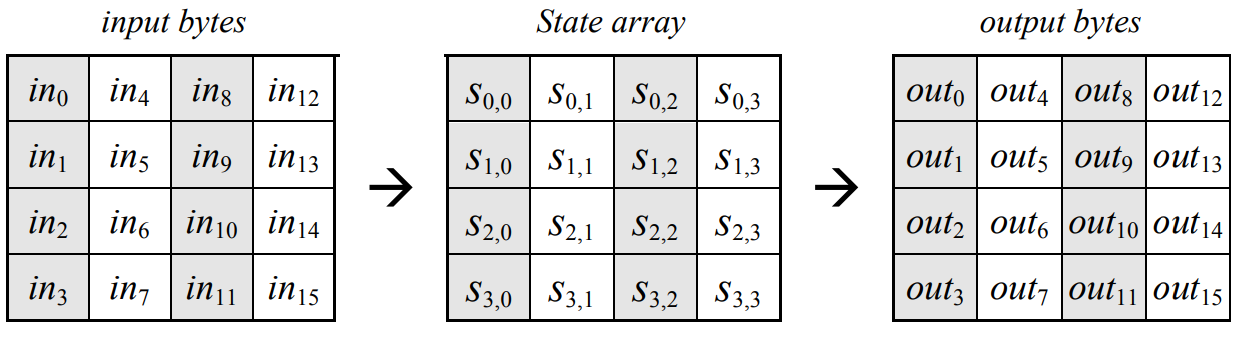
\includegraphics[width = \textwidth]{../Figures/FISP_AES/state.png} 
\caption[State array input and output.]{State array input and output. Source: \cite{nist197}.}\label{fig:AES_state}
\end{figure}

A description of the five functions is provided hereafter.

\subsubsection*{KeySchedule}
The key round of the initial round of AES coincides with the secret encryption key $\boldsymbol{K} = (k_{0,0},k_{0,1},\dots,k_{0,3}, k_{1,0},\dots,k_{1,3},\dots,k_{3,3})$. The $i$-th round key is given by 
\begin{equation*}
\boldsymbol{K_i} = (k_{4i,0},k_{4i,1},\dots,k_{4i,3}, k_{4i+1,0},\dots,k_{4i+1,3},\dots,k_{4i+3,3}),
\end{equation*}
where, for $i>3$
\begin{equation*}
\begin{cases}
k_{a,b} = k_{a-4,b}\oplus k_{a-1,b} & \mbox{if } a \not\equiv 0 \mbox{ mod } 4\\
k_{a,b} = k_{a-4,b}\oplus \Sbox(k_{a-1,(b+1) \mbox{mod } 4}) \oplus \mathrm{Rcon}(a) & \mbox{if } a \equiv 0 \mbox{ mod } 4 \mathrm{,}
\end{cases}
\end{equation*}

where $Rcon(a) = 2^{a-1}$ in the Rjindael finite field.\footnote{where $2=(00000010)_2$ is represented by the polynomial $x$}

\subsubsection*{AddRoundKey}
\subsubsection*{SubByte}
\subsubsection*{ShiftRow}
\subsubsection*{MixColumn}


\subsection{Description of RSA}


%----------------------------------------------------------------------------------------
%	SECTION 2
%----------------------------------------------------------------------------------------
\section{Secured Components}
\section{Smart Cards and Related Devices}
As we have seen in the previous section, modern cryptography proposes solutions to secure communications that ask for electronic computations and repose their security over some secret keys. Keys are represented as long bit strings, impossible to be memorized by users. Thus, keys need to be stored in a secure medium, and never delivered in clear over insecure channels. Smart cards were historically conceived as a practical solution to such a key storage issue: they consist in small devices a user can easily carry around with, which not only store secret keys, but also are able to internally perform cryptographic operations, in such a way that keys are never asked to be delivered. The registrations of a first patent by Roland Moreno in 1974 and of a second one by Michel Ugon in 1977 are often referred to date the smart card invention, finally produced for the first time in 1979. Smart cards are pocket-sized plastic-made cards equipped with a secured component, which is typically an integrated circuit containing a some computational units and some memories.\\

Today, about 40 years after its invention, they still have a huge diffusion, both in terms of applicative domains and in terms of quantity of exemplars. Indeed, they serve as credit or ATM cards, healthy cards, ID cards, public transport payment cards, fuel cards, identification and access badges, authorization cards for pay television, etc. Slightly changing the card support, we find other applications of the same kind of integrated circuits, for example the  mobile phone SIMs (\emph{Subscriber Identity Module} and the electronic passports. In terms of quantity, it seems that in 2014 8.8 billion smart cards have been sold, \emph{i.e.} the same order of magnitude of the global population. \\

In addition to smart cards, the recent growing and variation of security needs lead to the development and specification of other kinds of secured components, for example the \emph{Trusted Execution Environment} (TEE), which as a secured part of the main processor of a smartphone or tablet, and the \emph{Trusted Platform Module} 
(TPM), which is a secure element providing cryptographic functionalities to a motherboard. 

\subsection{Embedded Cryptography Vulnerabilities}
\subsubsection{Side-Channel Attacks}
Until the middle of nineties, the security of embedded cryptosystems was considered as equivalent to the mathematical security of the cryptographic algorithm. In classical cryptanalysis an attacker has usually the knowledge of the algorithm (in accordance to the Kerckhoff's principle) and of some inputs and/or outputs. Starting from this data, his goal is to retrieve the secret key. This attack model considers the algorithm computation as a black box, in the sense that no internal variable can be observed during execution, only inputs and/or outputs. With his seminal paper about Side-Channel Attacks (SCAs) in 1996, Paul Kocher showed that such a black-box model fails once the algorithm is implemented over a material component \cite{kocher1996timing}: an attacker can indeed inspect its component during the execution of the cryptographic algorithm, monitor some physical quantities, for example the execution time \cite{kocher1996timing} or the instantaneous power consumption \cite{kocher1999differential} and deduct information about internal variables of the algorithm. Depending on the attacked algorithm, making inference over some well chosen internal variable (the so-called \emph{sensitive variables} of the algorithm) is sufficient to retrieve the secret key. After these first works it was shown that other observable physical quantities contained \emph{leakages} of sensitive information, for example the electromagnetic radiation emanating from the device \cite{gandolfi2001electromagnetic,quisquater2001electromagnetic} and the acoustic emanations \cite{genkin2014rsa}. Moreover, if until few years ago it was thought that only small devices, equipped with slow microprocessors and in a small-size architecture, such as smart cards were vulnerable to this kind of Side-Channel Attacks, this recent work about acoustic emanations, together with other works exploiting electromagnetic fluctuations pointed out that much faster and bigger devices, \emph{i.e.} laptops and desktop computers, are vulnerable as well \cite{genkin2015stealing,genkin2015get,genkin2016ecdh}.

\subsubsection{A Classification of the Attacks to Secured Components}
\begin{table}[]
\centering
\caption{Classification of Attacks}
\label{fig:classification_attacks}
\begin{tabular}{|l|lll}
\cline{1-3}
\multirow{4}{*}{\textbf{Hardware Attacks}} & \multicolumn{1}{l|}{Passive} & \multicolumn{1}{l|}{Active} &                                    \\ \cline{2-4} 
                                           & \multicolumn{1}{l|}{}        & \multicolumn{1}{l|}{}       & \multicolumn{1}{l|}{Invasive}      \\ \cline{2-4} 
                                           & \multicolumn{1}{l|}{}        & \multicolumn{1}{l|}{}       & \multicolumn{1}{l|}{Semi-Invisive} \\ \cline{2-4} 
                                           & \multicolumn{1}{l|}{SCAs}    & \multicolumn{1}{l|}{FAs}    & \multicolumn{1}{l|}{Non-Invasive}  \\ \hline
\textbf{Software Attacks}                  &                              &                             &                                    \\ \cline{1-1}
\end{tabular}
\end{table}

The Side-Channel Attacks outlined in previous paragraph belong to a much bigger family of attacks that can be performed to break cryptographic devices security claims. First of all software attacks and hardware attacks must be distinguished. Software attacks only exploit vulnerability coming from the way the component's code is written. Hardware attacks are still commonly classified on the base of two criteria: on one hand we can distinguish passive and active attacks, on the other hand we can distinguish invasive, semi-invasive, non-invasive attacks. 
\begin{itemize}
\item[] \textbf{Passive attacks:} in passive attack, the device is let run respecting its specifications. The attacker observes its behaviour without provoking any alteration;
\item[] \textbf{Active attacks:}  in active attacks a special manipulation is performed in order to make the normal behaviour of the device change. 
\end{itemize}


\begin{itemize}
\item[] \textbf{Invasive attacks}: in invasive attack, the device is depackaged and inspected at the level of the components technology. The circuit can be modified, broken, signals can be accessed via a probing station, etc. There is no limits to the manipulations attacker can do to the components;
\item[] \textbf{Semi-invasive attacks}: as in invasive attacks the device is depackaged, but in contrast to them, no direct electrical contact to the chip is done;
\item[] \textbf{Non-invasive attacks}: in non-invasive attacks the device is not modified and only accessible interfaces are exploited. 

In literature, the term Side-Channel Attacks commonly denotes the passive non-invasive attacks. In the same way, active non-invasive attacks are often referred to as \emph{Fault Injection Attacks}. 

\end{itemize}

\subsection{Certification of a Secure Hardware}

parla anche degli attachi per perturbazione (tesi alexandre)


